\documentclass[11pt]{beamer}
\let\Tiny=\tiny
\let\epsilon=\varepsilon
\usepackage{amsmath}
\usepackage{amsfonts}
\usepackage{amssymb}
\usepackage{graphicx}
\usepackage{array}
\usepackage{tikz}
\usepackage{framed}

\definecolor{cherryred}{RGB}{214,31,74}
\definecolor{sandiasilver}{RGB}{204,204,204}
\definecolor{lightblue}{RGB}{240,245,255}

\usecolortheme[named=cherryred]{structure}
\usefonttheme[onlymath]{serif}
\setbeamertemplate{navigation symbols}{}
\setbeamertemplate{blocks}[shadow=true]
\setbeamersize{sidebar width left=0.2cm}
\setbeamercolor{sidebar}{bg=sandiasilver}
\setbeamercolor{frametitle}{fg=white, bg=cherryred}
\setbeamertemplate{theorems}[numbered]


\author{David E. Weirich}
\title{Neural Networks: \\ The Hard Way}
\date{\today}

\newcommand{\R}{\mathbb{R}}
\newcommand{\C}{\mathbb{C}}
\newcommand{\Z}{\mathbb{Z}}
\newcommand{\D}{\mathcal{D}}
\newcommand{\A}{\mathcal{A}}
\newcommand{\B}{\mathfrak{B}}
\newcommand{\Dh}{\tilde{\mathcal{D}}}

\newcommand{\supp}{\operatorname{Support}}
\newcommand{\ch}{\operatorname{ch}}
\newcommand{\proj}{\operatorname{Proj}}
\newcommand{\spn}{\operatorname{span}}
\newcommand{\quadr}{\operatorname{Quad}}
\newcommand{\qak}{Q_\alpha^k}
\newcommand{\one}{\textbf{1}} % Get the better looking one working!

\newcommand{\mean}[2]{\langle #2 \rangle_{#1}}

\newtheorem{conjecture}[theorem]{Conjecture}

\newcommand{\zak}{z_\alpha^k}

\newcommand{\bfred}[1]{{\color{cherryred} \textbf{#1}}}
\begin{document}

\begin{frame}
\titlepage
\end{frame}

\begin{frame}{Talk Objectives}

\begin{itemize}
\item Understand the mathematical basis for artificial neural networks.

\item Use that knowledge to design and build a neural network without relying on preexisting ML frameworks.
\end{itemize}

\bigskip

\pause

Or in other words...

\bigskip

\pause

\hspace{10mm}\textbf{Learn Neural Networks THE HARD WAY}

\end{frame}

\begin{frame}{Disclaimer}
\begin{center}
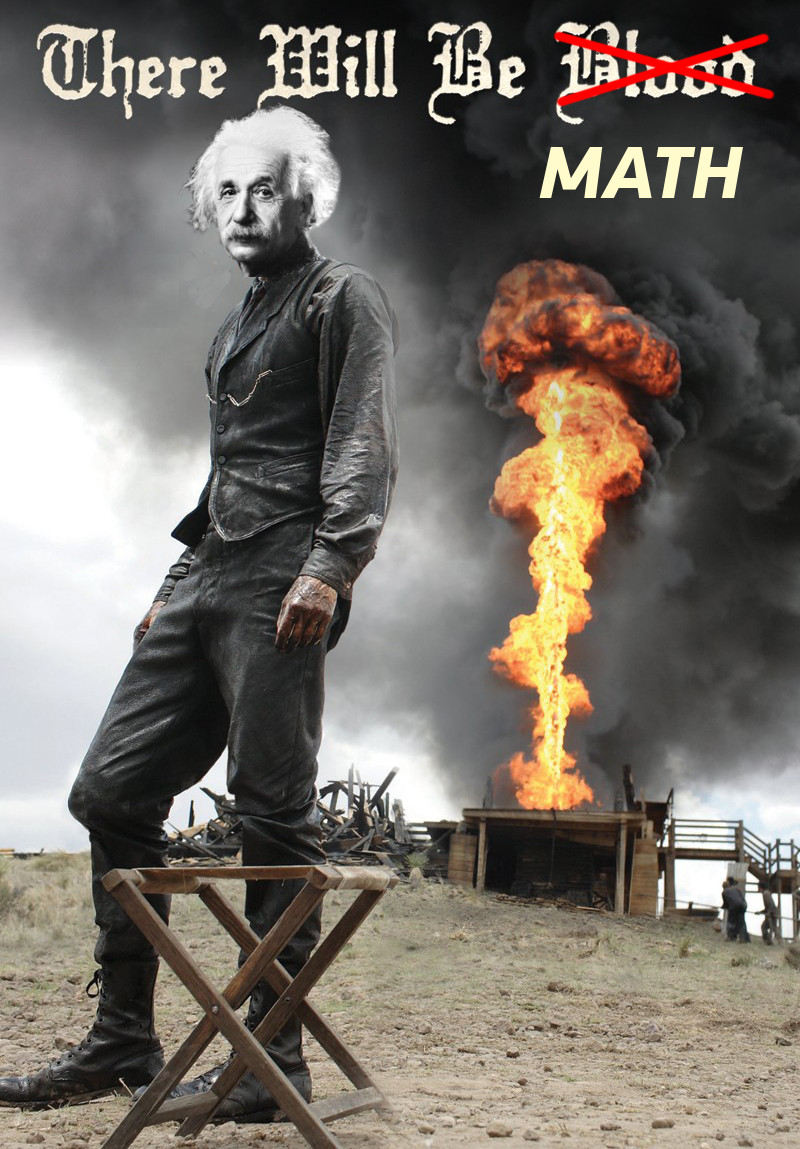
\includegraphics[scale=0.18]{ThereWillBeMath}
\end{center}
\end{frame}

\section{What are these Neural Networks Things?}

\begin{frame}{Why the ``hard way''??? I prefer easy!}

\emph{What do I mean by "the hard way"?}

\bigskip

\bigskip	

Doing things the hard way means teaching you how to teach yourself.

\end{frame}

\begin{frame}{The Problem}

We wish to approximate a function given a finite collection of known inputs and outputs.

\bigskip

$$||F - \widehat{F}|| < \epsilon$$

\bigskip

Here $F$ is the true function, and $\widehat{F}$ is our approximation.
\end{frame}

\begin{frame}{What are Neural Networks?}
\textbf{Q:} What is a neural network?

\bigskip 

\textbf{A:} \emph{A neural network is this super confusing thing that is kind of like an artificial brain.}

\bigskip 

\textbf{Q:} Why do we care?

\bigskip 

\textbf{A:} \emph{It can learn anything, do anything, and no one really understands them.}
\end{frame}

\begin{frame}{Neurons}

\begin{center}
\begin{figure}
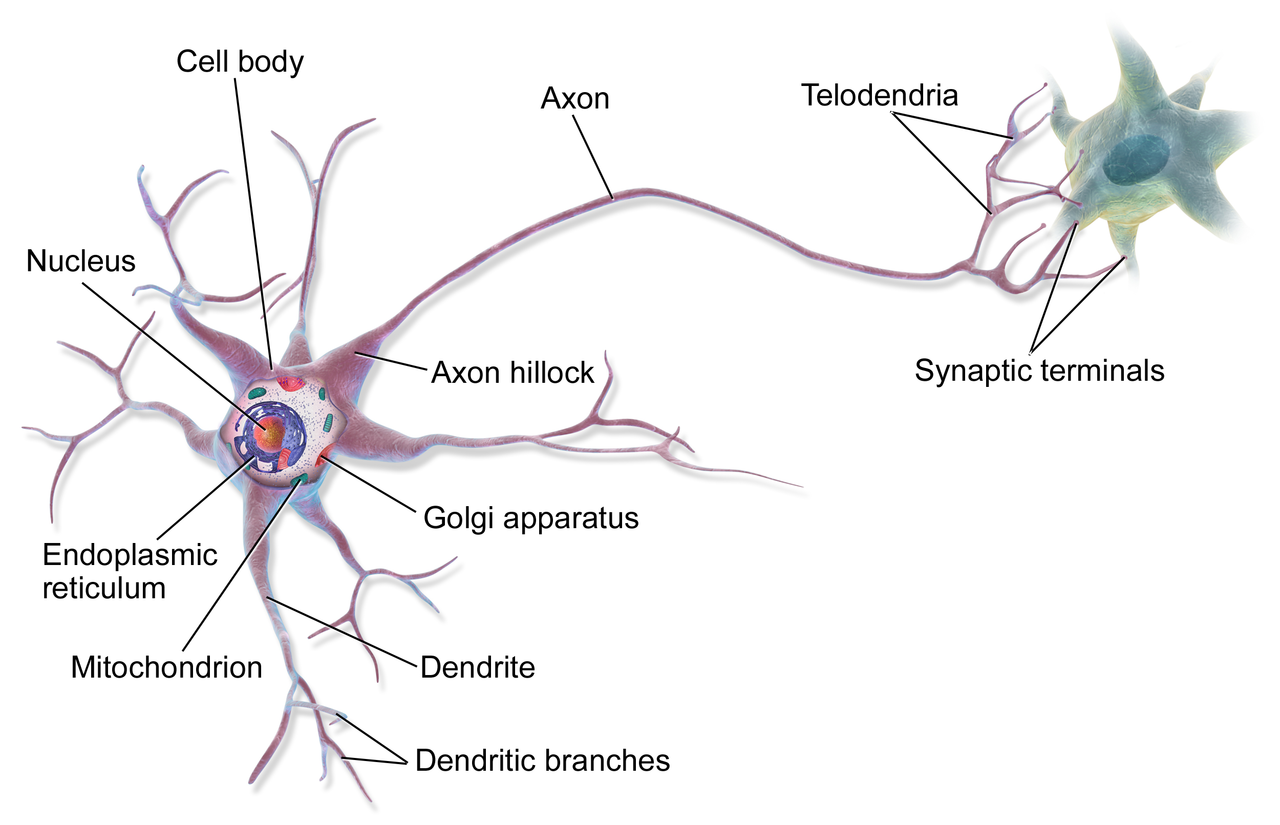
\includegraphics[scale=0.2]{Blausen_0657_MultipolarNeuron}
\caption{A neuron. These things are involved somehow?}
\end{figure}
\end{center}
	
\end{frame}

\begin{frame}{Pictures that look like this}

\begin{center}
\begin{figure}
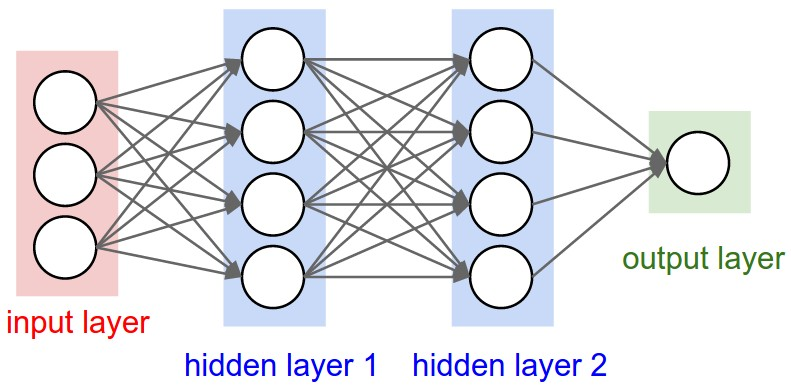
\includegraphics[scale=0.2]{0_IlHu39jf2c7QC4kn}
\hspace{5mm}
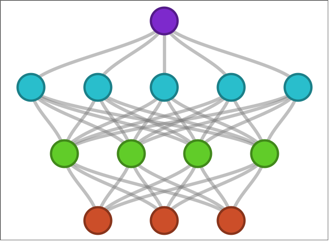
\includegraphics[scale=0.2]{topdown}

\vspace{5mm}

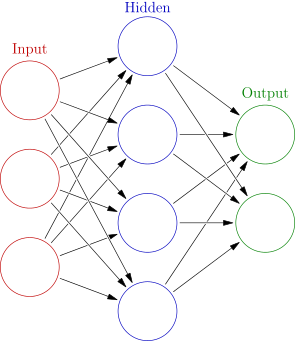
\includegraphics[scale=0.25]{296px-Colored_neural_network}
\hspace{5mm}
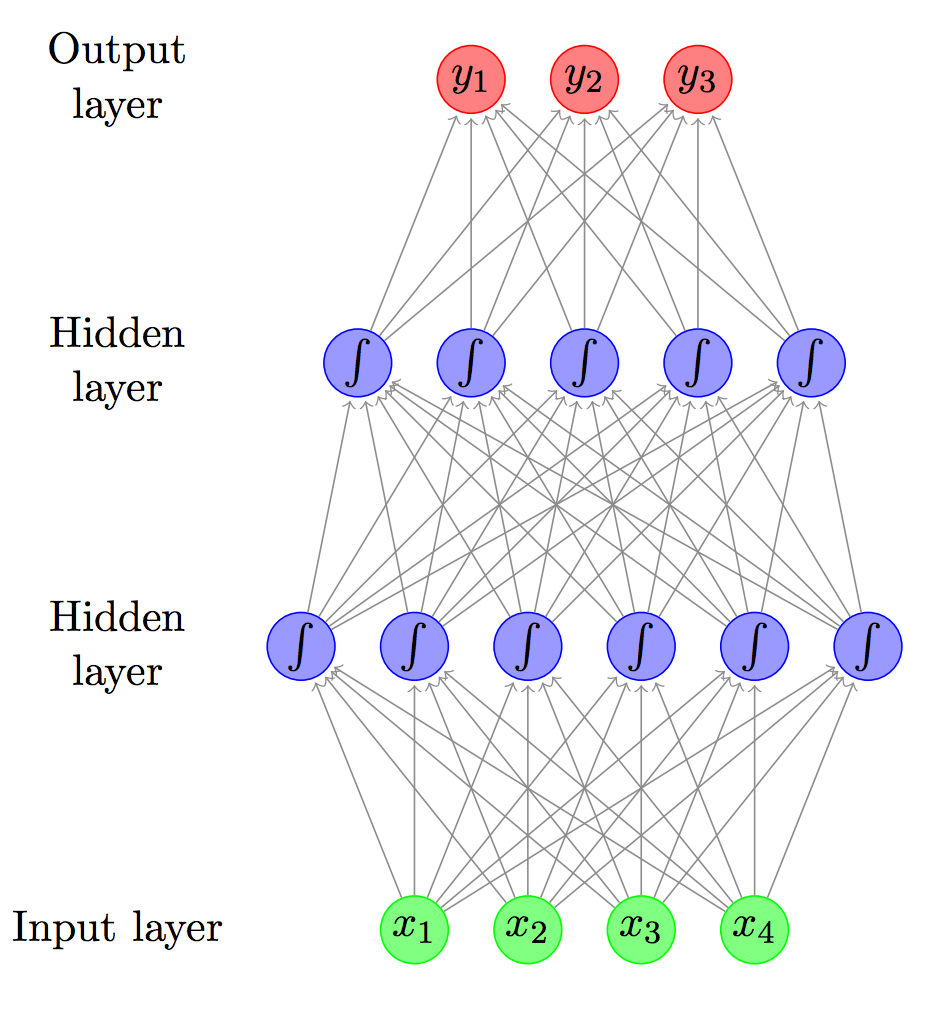
\includegraphics[scale=0.15]{Feed-forward-neural-network-with-two-hidden-layers}
\caption{Some diagrams with circles and arrows.}
\end{figure}
\end{center}

\end{frame}

\begin{frame}{A Motivating Example: Classifying Digits}
Suppose you were the kind of person who wanted to identify some pictures of numerical digits.

\begin{center}

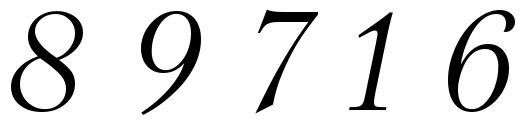
\includegraphics[scale=0.4]{digits}

\pause

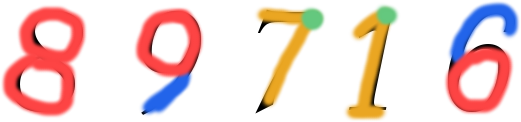
\includegraphics[scale=0.4]{digits2}

\pause

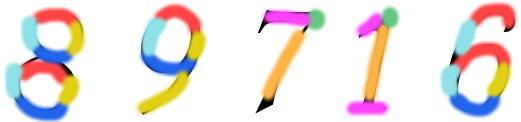
\includegraphics[scale=0.4]{digits3}

\end{center}
\end{frame}

\begin{frame}{The $\Sigma$exy Part of the Talk}
Let's take a look at the math under the hood:
\begin{align*}
x &= \left[\begin{array}{c}
x_1 \\
x_2 \\
\vdots \\
x_N
\end{array}\right] \\
\widehat{y} &= \widehat{F}(x) = W_2\sigma(W_1\sigma(W_0x + b_0) + b_1) + b_2
\end{align*}

where $W_i$ is a weight matrix, $b_i $ is a bias vector, and $\sigma$ is an activation function.
\end{frame}

\begin{frame}{Breaking that down}

Let's look at that again, step by step:

\begin{align*}
z_0 &:= W_0x + b_0 \\
a_0 &:= \sigma(z_0) \\
z_1 &:= W_1a_0 + b_1 \\
a_1 &:= \sigma(z_1) \\
&\vdots \\
\widehat{y} &:= W_n a_{n-1} + b_n
\end{align*}

\end{frame}

\begin{frame}{Universal Approximation Theorem}
\begin{theorem}[Cybenko (1989), Hornik (1991)]
Let $\sigma$ be a nonconstant, bounded, and monotonically increasing function.
Given any $\epsilon > 0$ and any continuous function $F$ defined on a compact subdomain $\Omega$ of $\R^n$ there exists a constant $N$, real constants $v_i$ and $b_i$, and real vectors $w_i$ such that we may define
$$\widehat{F}(x) := \sum_{i = 1}^N v_i \sigma(w_i^T \cdot x + b_i)$$
with
$$\left|F(x) - \widehat{F}(x)\right| < \epsilon$$
for all $x$ in $\Omega$.
\end{theorem}
\end{frame}

\section{Training}
\begin{frame}{Okay, fine, I get it. But how do I set those weights?}

For $M$ observations $(x_i, y_i)$, define a loss function

\begin{align*}
J(y_i, \widehat{y}) &:= \frac{1}{2M}\sum_{i =1}^N (y - \widehat{y})^2 \\
&= \frac{1}{2M}\sum_{i =1}^N \left(y - \widehat{F}(x_i)\right)^2 \\
&= \frac{1}{2M}\sum_{i =1}^N \left(y - \widehat{F}(x_i; W, b)\right)^2 
\end{align*}
Now we just have to minimize the loss!
\end{frame}

\begin{frame}{The Gradient}
Recall from multivariable calculus that the \emph{gradient} is a vector which points in the direction of steepest assent on a surface.
\begin{center}
\begin{figure}
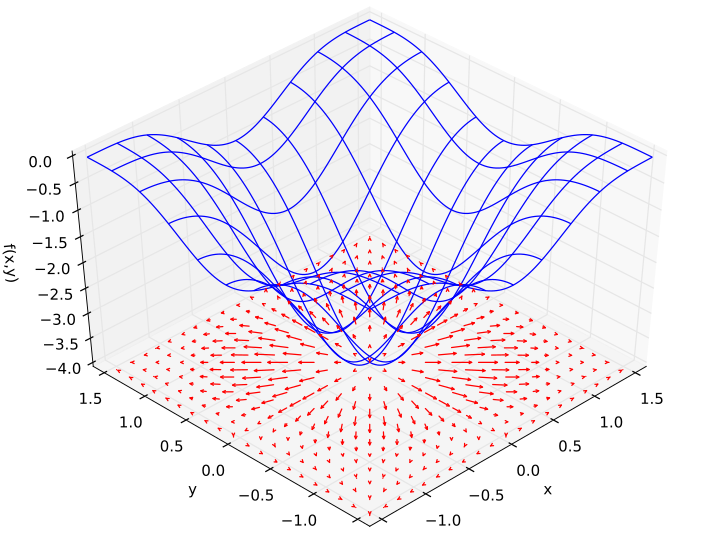
\includegraphics[scale=0.25]{720px-Gradient_Visual}
\caption{A function of two variables, with its gradient.}
\end{figure}
\end{center}
\end{frame}

\begin{frame}{Calculating the Gradient}

Normally we would use an algorithm called ``Back Propogation\footnote{Or as I like to call it, the chain rule with clever bookkeeping.}'' to calculate the gradients.

\bigskip

But I just did it this way:

\begin{center}
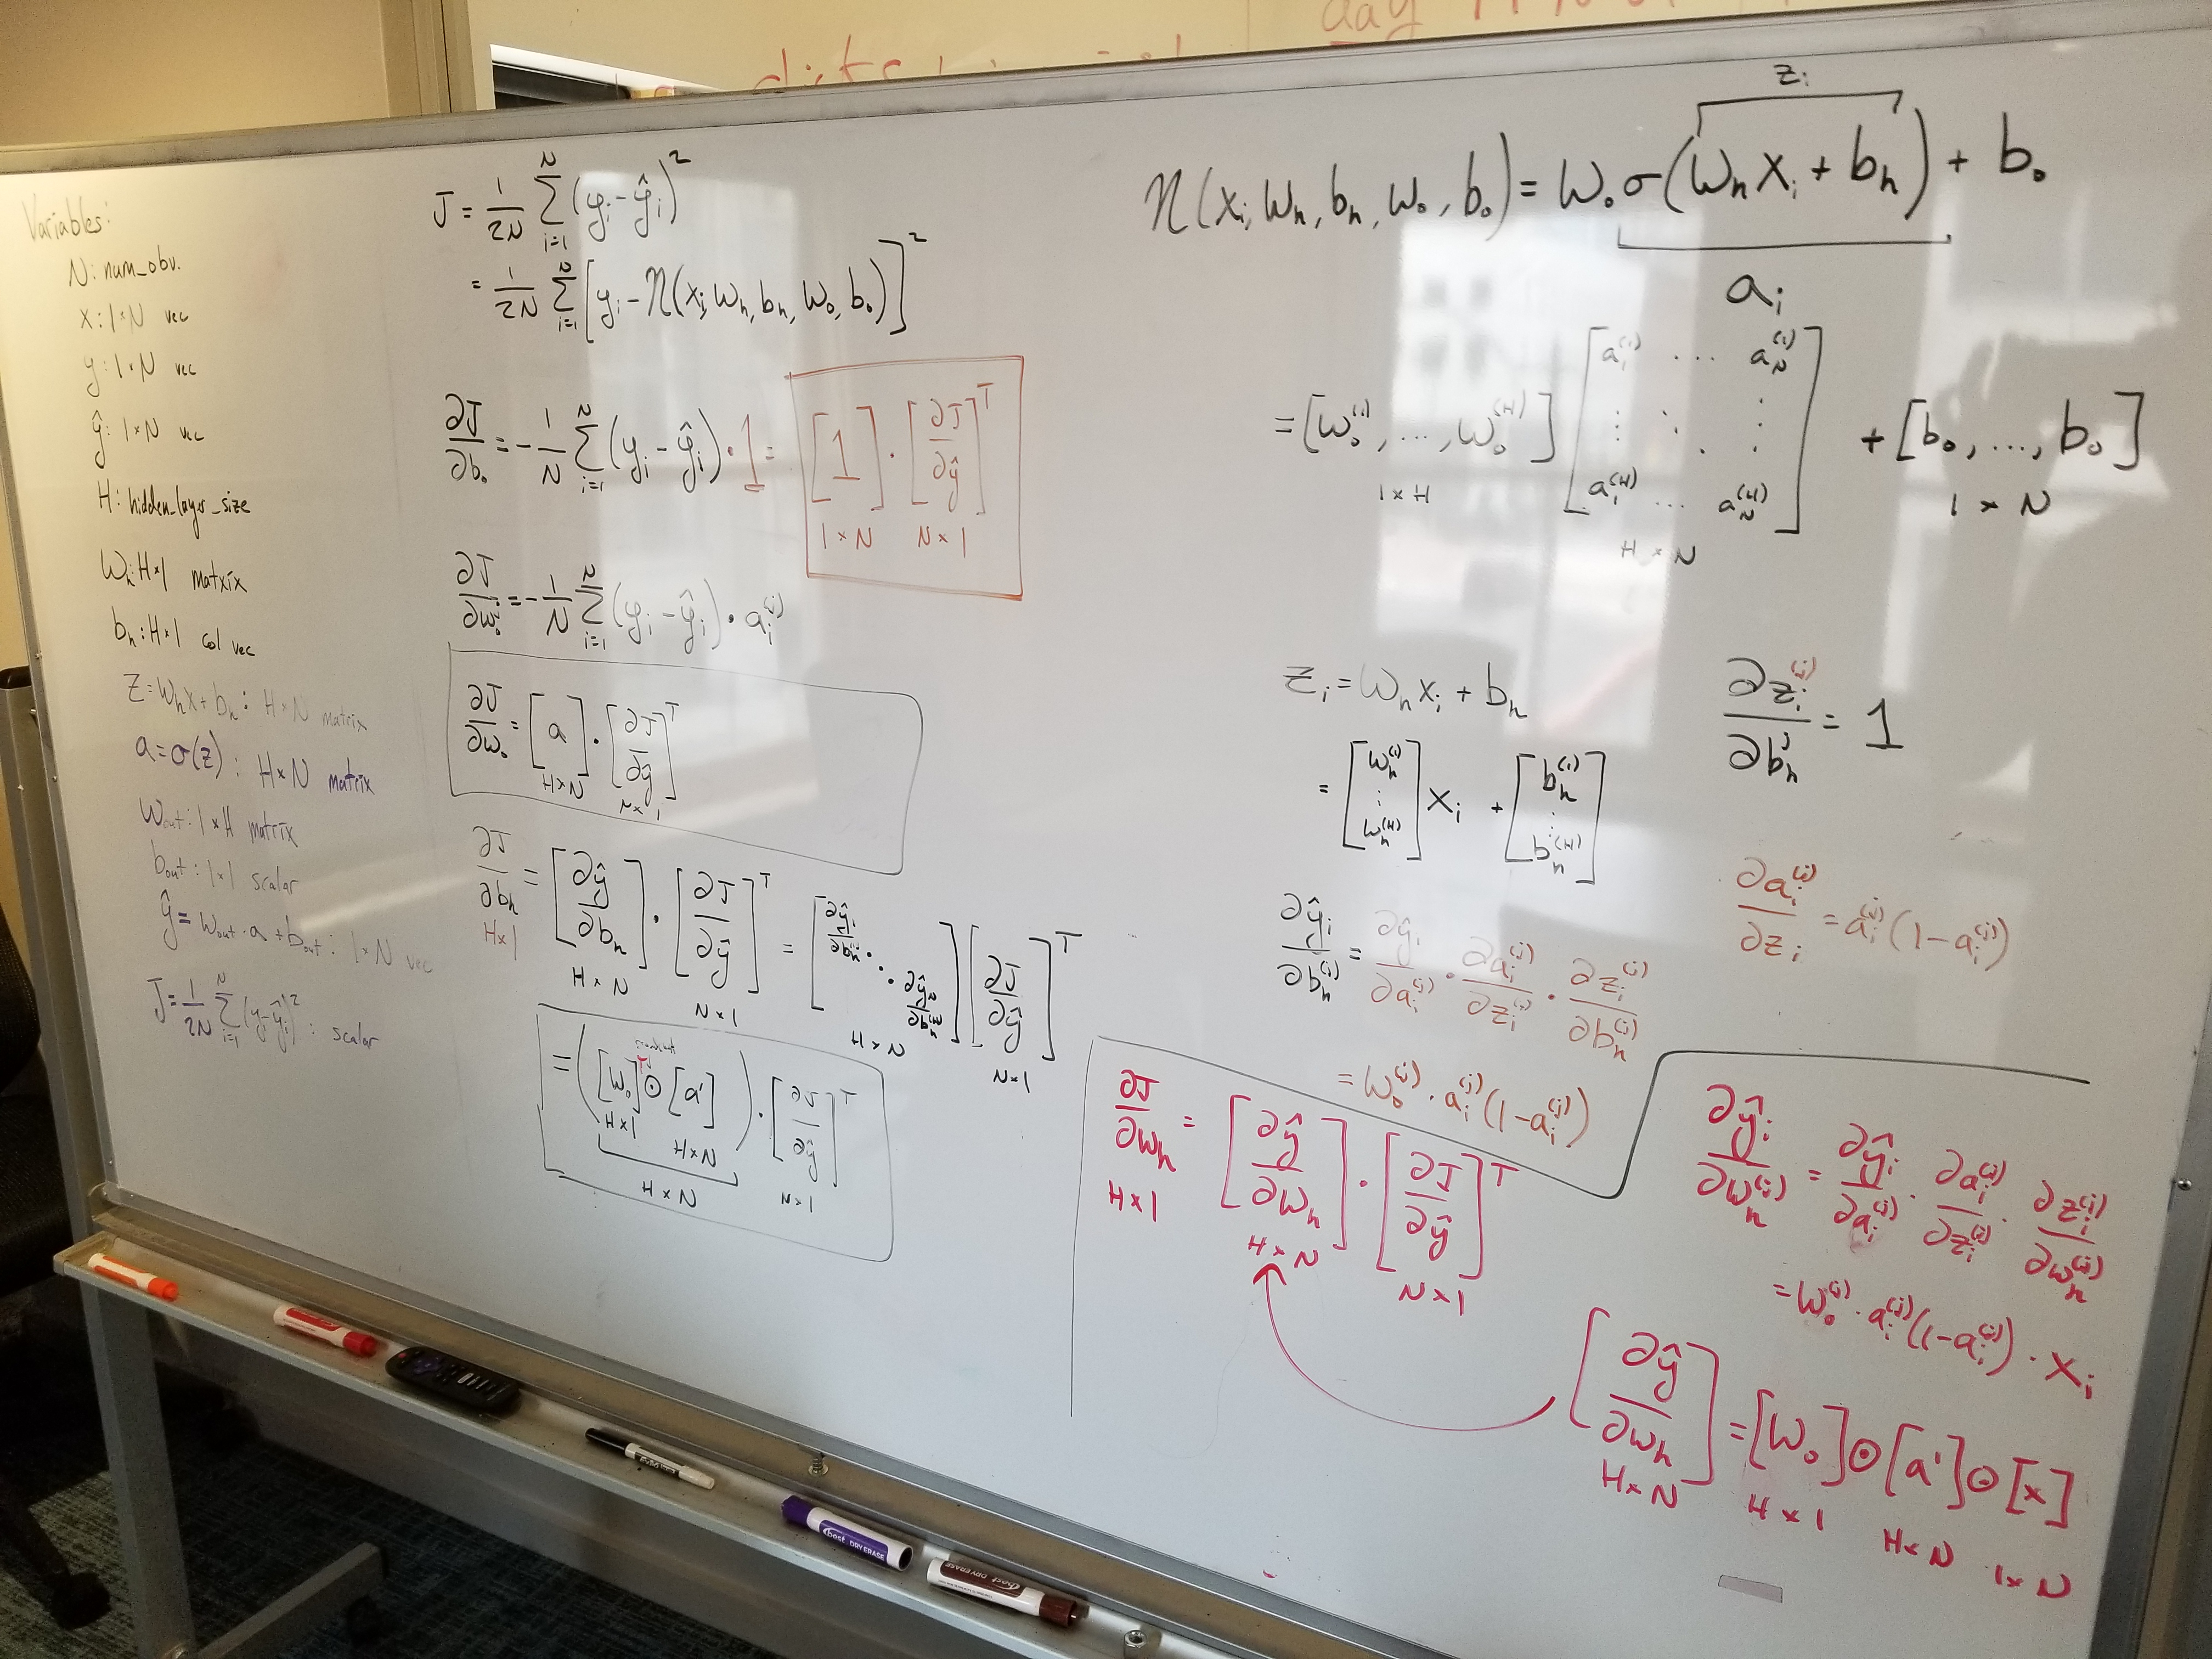
\includegraphics[scale=0.04]{20180305_112255}
\end{center}

\end{frame}

\begin{frame}{The Game Plan}
\begin{itemize}
\item We start by setting the weights and biases of the NN randomly.
\item Calculate the gradient of the loss function $J$ with respect to these parameters.
\item Update the parameters a tiny bit by taking a step in the direction of the negative gradient.
\item Repeat until the error is acceptable.
\end{itemize}
\end{frame}

\section{The Code}

\begin{frame}{WE'LL DO IT LIVE}
\begin{center}

\includegraphics[scale=0.3]{114486a48d800d14f972cb0e74f7b0d9}

WE'LL DO IT LIVE!
\end{center}
\end{frame}

\section{End}

\begin{frame}{Concluding Remarks}

\begin{itemize}
\item Neural networks are powerful because they combine the ability to approximate any function with a systematic method for improving that approximation.
\item The loss function measures how well a given NN matches the desired function.
\item Gradient descent is the process by which we slowly nudge the parameters of the network in the proper direction in an attempt to minimize the loss function.
\end{itemize}

\end{frame}

\begin{frame}
\begin{center}
Thank you! :)
\end{center}
\end{frame}

\end{document}
